\section{Neutrino Oscillations. History and Status}
\subsection{First Discovery and Confirmation}
History of the discovery of these phenomane is described in \cite{ref_Griffiths}, chapter 11. The first evidence of the neutrino oscillations had place in the Ray Davis's experiment in 1968 with solar neutrinos which registered number of neutrinos three times smaller then theoretically predicted. The phenomenon was called "solar neutrino problem". This experiment used Chlorino radiochemical detector neutrino interacted with chlorine-37 atom and converted it to argon-37 through the reaction $\nu_e+^{37}Cl \rightarrow ^{37}Ar+e$ or, at more fundamental level, $\nu_e+n \rightarrow p+e$. Then argon atoms were separated and counted. The detector was sensitive to electron neutrinos only. Soon after Bruno Pontecorvo proposed the explanation to the solar neutrino problem that neutrino can change it's flavor on it's way from the Sun to the detector. The theory was confirmed in 2001 by Super-Kamiokande collaboration. This experiment used water detector and could register any sort of neutrino though the $e+\nu \rightarrow e+\nu$ scattering. But the NC scattering can not distinguish between different neutrino flavors and also electron neutrinos could interact through CC which made detection efficiency of electron neutrinos 6.5 times higher than other flavors. \\

\begin{figure}
\caption{Schemes of the Solar neutrino experiments: Homestake Experiment, Super Kamiokande and Sudbury Neutrino Oscillations}
\label{fig:history_Schemes}
\centering
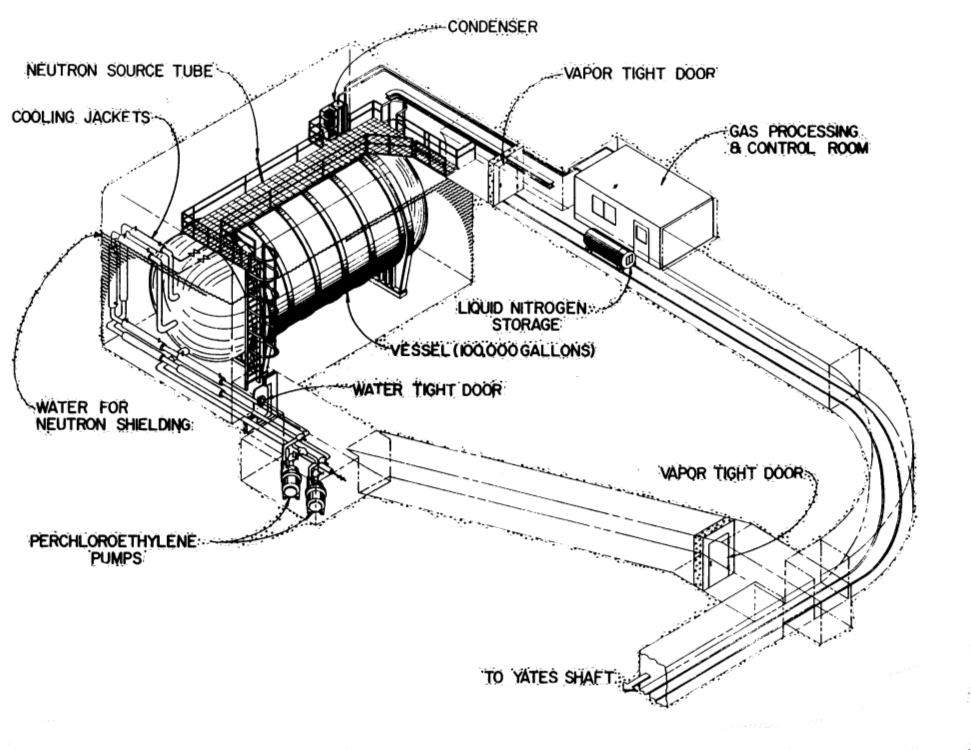
\includegraphics[width=0.80\textwidth, keepaspectratio=true]{figs/history_Homestake01.png}
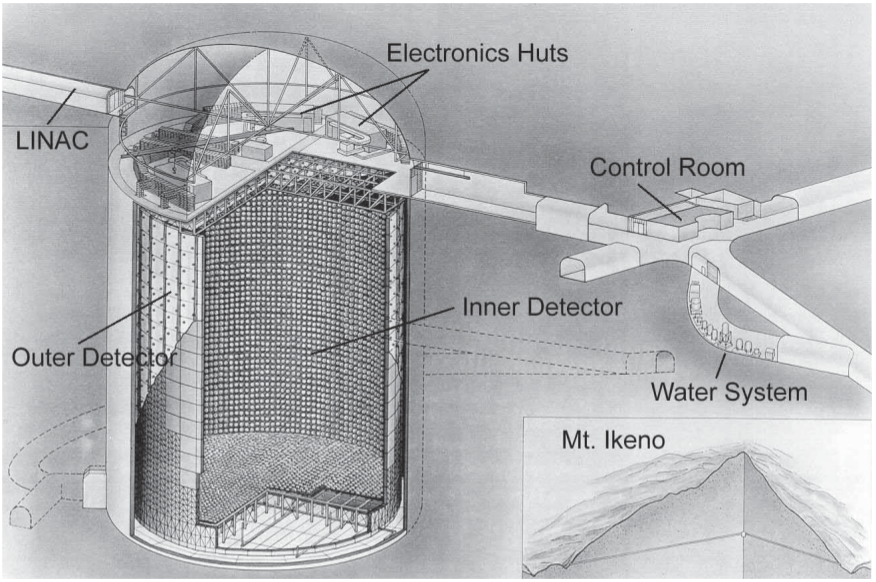
\includegraphics[width=0.50\textwidth, keepaspectratio=true]{figs/history_SuperK01.png}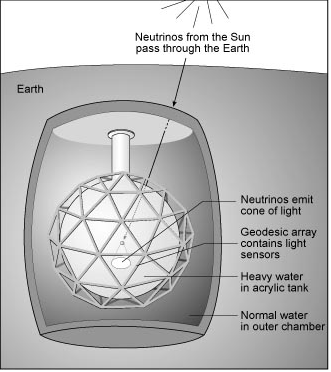
\includegraphics[width=0.30\textwidth, keepaspectratio=true]{figs/history_SNO01.png}
\end{figure}

\subsection{Neutrino Detection Techniques} 
Neutrinos can scatter on detector electrons throug weak neutral current (Z-boson). In this interaction, electron would leave the nuclei and would be detected. By measuring electron momentum and energy, it would be possible to receive information about original neutrino erergy and momentum but there would be no information about neutrino flavor. Also, neutrinos can interact through weak charged current ($W^\pm$-bosons) and produce charged lepton ($e^\pm$, $\mu^\pm$ or - if tau-neutrino is energetic enough - $\tau^\pm$). The properties of charged lepton can be measured in the detector and then from momentum and energy conseravation laws, the original neutrino properties will be reconstructed. Lepton flavor numbers are always conserved in these reactions and therefore it would be possible to determine the flavor of neutrino too (electron neutrino can only produce electron, muon neutrino can only produce muon and tau-neutrino can only produce tau-lepton).
The wikipedia page of Neutrino Detectors list the main detection techniques which make possible to register neutrinos \cite{ref_wiki_NeutrinoDetectors}:

\begin{figure}
\caption{Feynmann diagrams of neutral current (NC, left), and neutral current (CC, middle and right) neutrino scattering.}
\label{fig:MuonAndNeutronDecays}
\centering
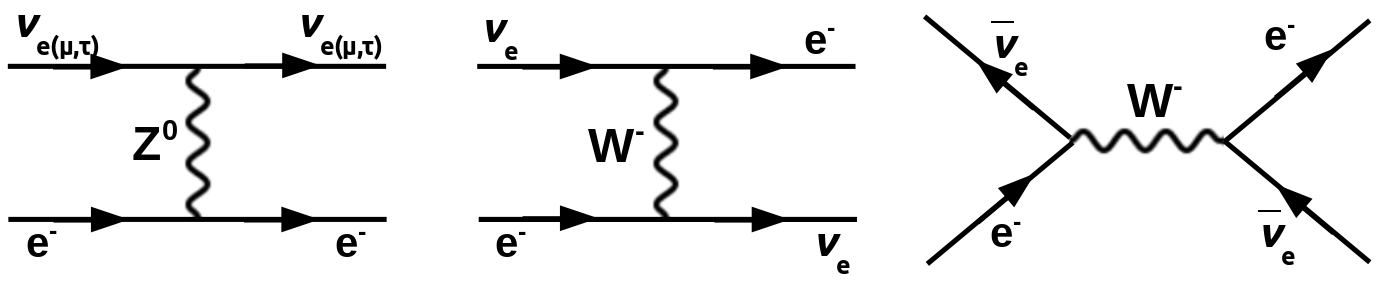
\includegraphics[width=0.9\textwidth, keepaspectratio=true]{figs/neutrinoScattering.png}
\end{figure}
\begin{itemize}

  \item Scintillators. Was used in the first experiment which registered antineutrinos - Savannah River nuclear reactor experiment. Water with cadmium chloride solution was used as a target. Antineutrinos from the reactor interacted with protons of the target as $\bar{\nu_e}+p \rightarrow n+e^+$. Then positron annilated with electron $e^+ + e^- \rightarrow \gamma + \gamma$ and the resulting photons are detected by scintillators. The neutron is captured by the cadmium nuclei with radiation of photon. This photon is also detected by the scintillator with delay of several microseconds. 
  \item Radiochemical methods. Chlorino radiochemical detector was used in south dakota experiment: neutrino interacted with chlorine-37 atom and converted it to argon-37. Then argon atoms were separated and counted. The experiment was the first to indicate the Solar Neutrino Problem. Same idea is used in certain experiments with gallium $\rightarrow$ germanium trasformation. The radiochemical methods are only useful for counting neutrinos but can't measure their kinematic characteristics.
  \item Cherenkov detectros. A charged particle travelling through the medium with speed $v>c/n$ where $c/n$ - is speed of light in this medium radiate photons which are called Cherenkov radiation. In general, this is threshold type of detection - particle is either detected or not. However, by having several layers with different n (refractive index), it's possible to differentiate charged particles by velocities better. Common working substance for Cherenkov detectors in neutrino physics are ice, water and heavy water.
  \item Tracking calorimeters. For high energy neutrinos, neutral current weak interactions cause hadronic shower and charged current weak interactions cause electromagnetic shower. The showers produced by charged particle (product of original neutrino nteraction) identify track parameters, momentum and energy of charged particle.
\end{itemize}


\subsection{Neutrino Oscillations}
Lets consider two neutrinos case as it's described in Griffiths\cite{ref_Griffiths}.\\*
Suppose there are only two neutrinos $\nu_e$ and $\nu_{\mu}$. Then true stationary states of the system would be the orthogonal combinations:\\*
$\nu_1=\nu_{\mu}cos\theta-\nu_esin\theta$\\*
$\nu_2=\nu_{\mu}sin\theta+\nu_ecos\theta$\\*
Then, according to the quantum mechanics,\\*
$\nu_1(t)=\nu_1(0)e^{\frac{-iE_1t}{h}}$, $\nu_2(t)=\nu_2(0)e^{\frac{-iE_2t}{h}}$\\*
Suppose, at t=0 there were $\nu_e(0)=1$, $\nu_\mu(0)=0$\\*
Then $\nu_1(0)=-sin\theta$, $\nu_2(0)=cos\theta$, $\nu_1(t)=-{sin\theta}e^{\frac{-iE_1t}{h}}$, $\nu_2(t)=-{cos\theta}e^{\frac{-iE_2t}{h}}$\\*
Thus, we are getting the system:\\*
$-{sin\theta}e^{-{{iE_1t} \over h}}=\nu_\mu(t)cos\theta-\nu_e(t)sin\theta$,\\*
$-{sin\theta}e^{-{{iE_2t} \over h}}=\nu_\mu(t)sin\theta-\nu_e(t)cos\theta$\\*
By solving this sytem for $\nu_e$ and $\nu_\mu$, one would get\\*
$P_{\nu_e \rightarrow \nu_\mu}=|\nu_\mu(t)|^2=[{sin2\theta}sin{\frac{(E_1-E_2)t}{2h}}]^2$,\\*
$P_{\nu_e \rightarrow \nu_e}=|\nu_e(t)|^2=1-[{sin2\theta}sin{\frac{(E_1-E_2)t}{2h}}]^2$\\*
Thus, for freely travelling neutrinos, if $\nu_e$ was emmitted, at any point there is a certain probability to register $\nu_e$ or $\nu_\mu$ and those probablities change with time periodically, by $~[sin(At)]^2$ law. That's why the phenomenon is called the neutrino oscillations.
Suppose momenta $p_1=p_2$. Then using $E^2=p^2+m^2$ and assuming $m_{1,2}<<E_{1,2}$, the probablities will take forms of\\*
$P_{\nu_e \rightarrow \nu_\mu}=|\nu_\mu(t)|^2=[{sin2\theta}sin{\frac{(E_1-E_2)t}{2h}}]^2$,\\*  

Three neutrino case is described in the "Long-baseline Neutrino Oscillation Physics" section of the draft Conteptual Design Report of the LBNF. For three neutrino case, the oscillations are determined by complex unitary matrix which is called Pontecorvo-Maki-Nakagava-Sakata (PMNS) matrix:\\*

$ \begin{pmatrix} \nu_{e} \\ \nu_{\mu} \\ \nu_{\tau} \\ \end{pmatrix}
 = U_{PMNS}\cdot \begin{pmatrix} \nu_{1} \\ \nu_{2} \\ \nu_{3} \\ \end{pmatrix} = 
 \begin{pmatrix}
  U_{e1} & U_{e2} & U_{e3} \\
  U_{\mu1} & U_{\mu2} & U_{\mu3} \\
  U_{\tau1} & U_{\tau2} & U_{\tau3} \\
 \end{pmatrix}
 \cdot
\begin{pmatrix} \nu_{1} \\ \nu_{2} \\ \nu_{3} \\ \end{pmatrix}$\\*

The $U_{PMNS}$ matrix depends on three neutrino mixing angles ($\theta_{12}$, $\theta_{23}$, $\theta_{13}$) and CP-violating phase $\delta_{CP}$. If define $c_{ab}=cos\theta_(ab)$, $s_{ab}=sin\theta_(ab)$, the $U_{PMNS}$ matrix can be splitted into three multipliers, each would be responsible for mixing of one pair of neutrino flavors:\\*

$U_{PMNS} =
 \begin{pmatrix}
  1 & 0 & 0 \\
  0 & c_{23} & s_{23} \\
  0 & -s_{23} & c_{23} \\
 \end{pmatrix}
 \cdot
 \begin{pmatrix}
  c_{13} & 0 & e^{i\delta_{CP}}s_{13} \\
  0 & 1 & 0 \\
  -e^{i\delta_{CP}}s_{13} & 0 & c_{13} \\
 \end{pmatrix}
 \cdot
 \begin{pmatrix}
  c_{12} & s_{12} & 0 \\
  -s_{12} & c_{12} & 0 \\
  0 & 0 & 1 \\
 \end{pmatrix}$ \\*

The probability amplitudes of neutrino mixing are defined by parameters of the $U_{PMNS}$ but, analogous to simplified two-neutrino case described above, the differences of squares of neutrino masses also contribute to the probability. There are two independent expressionce for sqares of masses differences: ${\Delta}m_{12}^2 = m_1^2-m_2^2$ and ${\Delta}m_{32}^2 = m_3^2-m_2^2$. Mass differences were measured in other neutrino oscillation experiments but the ${\Delta}m_{12}^2$ and ${\Delta}m_{32}^2$ present in the equations evenly and therefore the signs of these expressions were not measured. If the masses order as $m_3 > m_2 > m_1$, it's called normal neutrino mass hierarchy because other fundamental particles orders in a way that later generation particles have higher masses than lower generation particles. If the masses order as $m_1 > m_2 > m_3$ it's called inverted neutrino mass hierarchy. The mixing angles $\theta_{12}$, $\theta_{23}$, $\theta_{13}$ and differences of squared masses ${\Delta}m_{12}^2$ and ${\Delta}m_{32}^2$ are measured and give $U_{PMNS}$ matrix form of\\*

$|U_{PMNS}| \sim
 \begin{pmatrix}
  0.8 & 0.5 & 0.2 \\ 0.5 & 0.6 & 0.6 \\ 0.2 & 0.6 & 0.8 \\
 \end{pmatrix}$\\*

The CP-violating phase $\delta_{CP}$ is unknown.\\*
The analogous matrix for quark mixing, Cabibbo–Kobayashi–Maskawa (CKM) matrix, is much more diagonal:\\*

$|V_{CKM}| \sim
 \begin{pmatrix}
  1 & 0.2 & 0.004 \\ 0.2 & 1 & 0.04 \\ 0.008 & 0.04 & 1 \\
 \end{pmatrix}$\\*

One of the important questions in modern particle physics is why the quark mixing angles are so much smaller than neutrino mixing angles and the other important question is whether there is any relationship between quark and neutrino mixing matrices.\\*

The [REFERENCE] gives the following expression for $\nu_\mu \rightarrow \nu_e$ probability in presence of the Earth matter assuming it has constant density: \\*

$P(\nu_\mu \rightarrow \nu_e) \simeq sin^2{\theta_{23}}sin^2{2\theta_{13}}\frac{sin^2(\Delta_{13}-aL)}{(\Delta_{13}-aL)^2}\Delta^2_{31}+ \\*
+sin2\theta_{23}sin2\theta_{13}sin2\theta_{12}\frac{sin(\Delta_{31}-aL)}{(\Delta_{31}-aL)}\Delta_{31}\frac{sin(aL)}{aL}\Delta_{21}cos(\Delta_{31}+\delta_{CP})+ \\*
+cos^2\theta_{23}sin^2{2\theta_{12}}\frac{sin^2(aL)}{(aL)^2}\Delta^2_{21}$\\*

where $\Delta_{ij}={\Delta}m^2_{ij}L/4E$, and $a={G_F}{N_e}/sqrt(2)$\\*

For $P(\bar{\nu_\mu} \rightarrow \bar{\nu_e})$ one would need to change $\delta_{CP} \rightarrow -\delta_{CP}$ (bacuuse of neutrino-antineutrino assymetry for CP-violationg phase) and $a \rightarrow -a$ (because only electrons present in the Earth, not positrons). The effect of $a \rightarrow -a$ increases with L which means more sensitivity to mass hierarchy for experiments with larger baseline. The DUNE's baseline is 1300 km and it's expected to be enough to determine the neutrino mass hierarchy and also the CP-violation phase.

\begin{figure}
\caption{$P(\nu_\mu \rightarrow \nu_e)$ at a baseline of 1300 km}
\label{fig:LBNF_oscProbability}
\centering
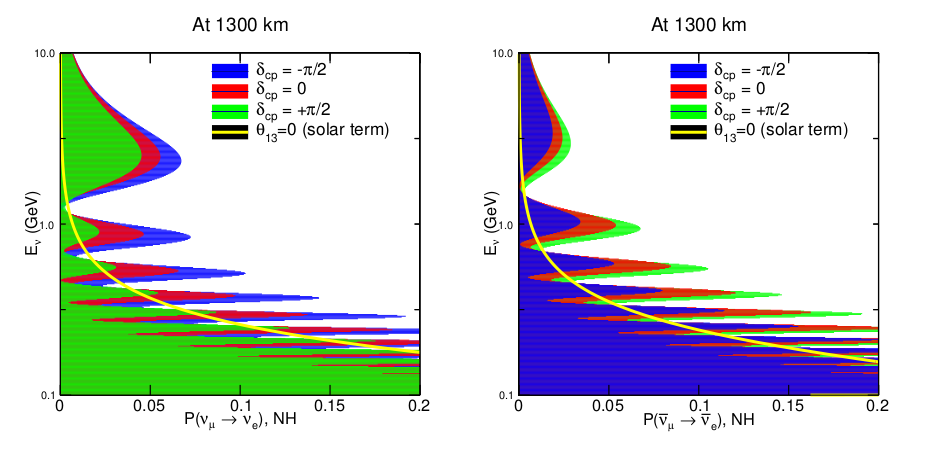
\includegraphics[width=0.98\textwidth, keepaspectratio=true]{figs/LBNF_oscProbability.png}
\\$P(\nu_\mu \rightarrow \nu_e)$ at a baseline of 1300 km, as a function of neutrino energy. Left - neutrinos, right - antineutrinos. Source of figure[REFERENCE]
\end{figure}

The figure\ref{fig:LBNF_oscProbability} shows that magnitude and frequency of oscillations both depend on $\delta_{CP}$ and the differences become more significant for higher oscillation nodes which correspond to lower energies of neutrino/antineutrino. Since changes due to different $\delta_{CP}$s are opposite for neutrinos and antineutrinos, it's important for the experiment to operate both.\\*

\subsection{Neutrino oscillation parameters measured in the other experiments}
The neutrino oscillation parameters measured in other experiments are summarized in the table \ref{tab:MeasuredPars} as quoted in the PDG[REFERENCE]:\\*
\begin{table}[h]
  \begin{center}
  \caption{ Neutrino oscillation parameters measured in other experiments}
  \begin{tabular}{|c|c|c|c|}
     Parameter & Value and uncerntainty & Experiment(s) \\ \hline
     $sin^2(2\theta_{12})$ &  $0.846\pm0.021$  &  KamLAND + global solar + SBL +accelerator: 3$\nu$  \\ \hline 
     $sin^2(2\theta_{23})$ &  $0.999^{+0.001}_{-0.018}$  &  T2K (if normal mass hierarchy)   \\ \hline 
     $sin^2(2\theta_{23})$ &  $1.000^{+0.000}_{-0.017}$  &  T2K (if inverted mass hierarchy)   \\ \hline 
     $sin^2(\theta_{13}), 10^{-2}$ &  $9.3\pm0.8$  &  DayaBay, Chooz, Yonggwang    \\ \hline 
     ${\Delta}m^2_{21}$, $10^{-5} eV^2$ &  $7.53\pm0.18$  &  KamLAND + global solar + SBL +accelerator: 3$\nu$   \\ \hline 
     ${\Delta}m^2_{32}, 10^{-3} eV^2$ &  $2.44\pm0.06$  &  T2K, MINOS, DAYA(if normal mass hierarchy)     \\ \hline
     ${\Delta}m^2_{32}, 10^{-3} eV^2$ &  $2.52\pm0.07$  &  T2K, MINOS, DAYA (if inverted mass hierarchy)     \\ \hline 
  \end{tabular}
  \label{tab:MeasuredPars}
  \end{center}
\end{table}

Section 14.5 in [REFERENCE] describes measurements of $\Delta{m^2_A}$ and $\theta_A$, splitting between atmospheric neutrino and accelerator experiments results. Section 14.6 reviews measurements of $\theta_{13}$ which was measured recently.

\subsection{Overview of Open Questions in Neutrino Physics} 
According Particle Data Group Review \ref{ref_PDG} the following questions will be the main priority to answer by current and future neutrino experiments:
\begin{itemize}
  \item whether the massive neutrinos are Dirac or Majorana (Dirac neutrinos are... Majorana neutrinos are...)
  \item what is the sign of $\Delta{m_A}^2$ ($\Delta{m_31}^2$) and what is the type of the neutrino mass spectrum [WHAT IS THAT]
  \item what the absolute values of neutrino masses are
  \item what is the value of the neutrino mixing angle $\theta_{13}$
  \item how does the CP-symmetry behaves in the lepton sector
  \item what the values of $\Delta{m_{12}}^2$, $\theta_{12}$, and $|\Delta{m_{31}}^2|$, $\theta_{23}$.
  \item are the neutrino oscillations indication of new fundamental symmetry in particle physics
  \item what is the relation between neutrino and quark mixing if any
  \item what is the nature of the CP-violation terms in the neutrino mixing matrix
  \item can better understanding of neutrino mixing give a hint to baryon assymetry in the Universe 
\end{itemize} 
